\documentclass[a4paper,11pt]{article}
\usepackage[utf8]{inputenc}\usepackage[T1]{fontenc}
\usepackage[english]{babel}\usepackage{lmodern}\usepackage{microtype}
\usepackage{amsmath,amssymb}\usepackage{geometry}
\geometry{a4paper,left=2.2cm,right=2.2cm,top=2.0cm,bottom=2.0cm}
\usepackage{booktabs,array}\usepackage{xcolor}
\definecolor{bokug}{RGB}{0,135,60}\usepackage{tikz}
\usetikzlibrary{arrows.meta,calc}
\usepackage{fancyhdr}\pagestyle{fancy}
\renewcommand{\headrulewidth}{0.4pt}
\usepackage{enumitem}\setlength{\parindent}{0pt}\setlength{\parskip}{4pt}

\begin{document}
\fancyhead[L]{\small VU Mechanik – LAWI 100515 (PI)}\fancyhead[R]{\small SS 2026}\fancyfoot[C]{\thepage}
\begin{center}{\large\bfseries\color{bokug}University of Natural Resources and Life Sciences, Vienna (BOKU)}\\[2pt]{\large\bfseries VU Mechanik – LAWI 100515 (PI)}\\[4pt]Exam \textbf{Group A} \hfill Date: 26.06.2026\\[2pt]\rule{\linewidth}{0.4pt}\end{center}

\begin{center}\textbf{\large Model solution}\end{center}
\begin{center}
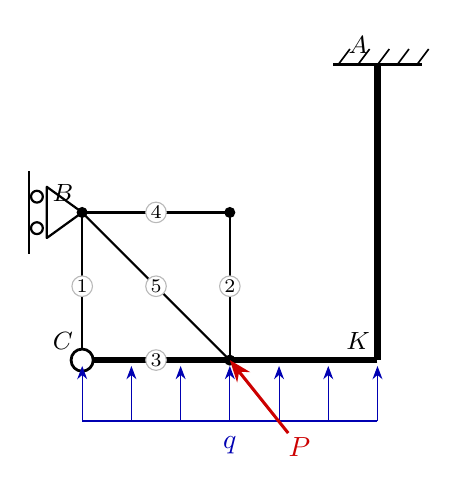
\begin{tikzpicture}[scale=1.250,>=Stealth,line join=round]
  \coordinate (P0) at (0.000,0.000);
  \coordinate (K) at (0.000,-3.000);
  \coordinate (C) at (-3.000,-3.000);
  \coordinate (TO1) at (-3.000,-1.500);
  \coordinate (TU0) at (-1.500,-3.000);
  \coordinate (TU1) at (-1.500,-1.500);
  \draw[thick] (C) -- (TO1);
  \draw[thick] (TU0) -- (TU1);
  \draw[thick] (C) -- (TU0);
  \draw[thick] (TO1) -- (TU1);
  \draw[thick] (TU0) -- (TO1);
  \draw[line width=2.2pt] (P0) -- (K);
  \draw[line width=2.2pt] (K) -- (C);
  \fill (C) circle (1.6pt);
  \fill (TO1) circle (1.6pt);
  \fill (TU0) circle (1.6pt);
  \fill (TU1) circle (1.6pt);
  \draw[fill=white,line width=1pt] (C) circle (3.2pt);
  \draw[line width=1.1pt] (0.450,0.000) -- (-0.450,0.000);
  \draw[line width=0.6pt] (0.400,0.000) -- (0.520,0.160);
  \draw[line width=0.6pt] (0.200,0.000) -- (0.320,0.160);
  \draw[line width=0.6pt] (0.000,0.000) -- (0.120,0.160);
  \draw[line width=0.6pt] (-0.200,0.000) -- (-0.080,0.160);
  \draw[line width=0.6pt] (-0.400,0.000) -- (-0.280,0.160);
  \draw[thick] (-3.000,-1.500) -- (-3.360,-1.240) -- (-3.360,-1.760) -- cycle;
  \draw[thick] (-3.460,-1.340) circle (0.06) (-3.460,-1.660) circle (0.06);
  \draw[line width=1pt] (-3.540,-1.080) -- (-3.540,-1.920);
  \node[circle,fill=white,draw=gray!55,inner sep=0.5pt,font=\scriptsize] at (-3.000,-2.250) {1};
  \node[circle,fill=white,draw=gray!55,inner sep=0.5pt,font=\scriptsize] at (-1.500,-2.250) {2};
  \node[circle,fill=white,draw=gray!55,inner sep=0.5pt,font=\scriptsize] at (-2.250,-3.000) {3};
  \node[circle,fill=white,draw=gray!55,inner sep=0.5pt,font=\scriptsize] at (-2.250,-1.500) {4};
  \node[circle,fill=white,draw=gray!55,inner sep=0.5pt,font=\scriptsize] at (-2.250,-2.250) {5};
  \draw[->,blue!70!black] (0.000,-3.620) -- (0.000,-3.060);
  \draw[->,blue!70!black] (-0.500,-3.620) -- (-0.500,-3.060);
  \draw[->,blue!70!black] (-1.000,-3.620) -- (-1.000,-3.060);
  \draw[->,blue!70!black] (-1.500,-3.620) -- (-1.500,-3.060);
  \draw[->,blue!70!black] (-2.000,-3.620) -- (-2.000,-3.060);
  \draw[->,blue!70!black] (-2.500,-3.620) -- (-2.500,-3.060);
  \draw[->,blue!70!black] (-3.000,-3.620) -- (-3.000,-3.060);
  \draw[blue!70!black,thick] (0.000,-3.620) -- (-3.000,-3.620);
  \node[blue!70!black] at (-1.500,-3.870) {$q$};
  \draw[->,red!80!black,line width=1.1pt] (-0.907,-3.742) -- (-1.500,-3.000);
  \node[red!80!black] at (-0.794,-3.882) {$P$};
  \node[font=\small] at (0.000,0.000) [xshift=-7pt,yshift=7pt] {$A$};
  \node[font=\small] at (0.000,-3.000) [xshift=-7pt,yshift=7pt] {$K$};
  \node[font=\small] at (-3.000,-3.000) [xshift=-7pt,yshift=7pt] {$C$};
  \node[font=\small] at (-3.000,-1.500) [xshift=-7pt,yshift=7pt] {$B$};
\end{tikzpicture}
\end{center}
\par\medskip\textbf{1.\ Static determinacy}\par Counting criterion $n=3k-(a+z)$ (bodies $k$, reactions $a$, interaction forces $z$):
\[ n=3k-(a+z)=3\cdot2-(4+2)=0\ \Rightarrow\ \text{statically determinate} \]
\par\medskip\textbf{2.\ Support reactions and hinge forces}\par
$A:\ R_x=-2,\ R_y=-25,\ M=46.5$\quad $B:\ R_x=10,\ R_y=0$\par $C:\ H_x=2,\ H_y=10$
\par\medskip\textbf{3.\ Truss member forces}\par
\begin{center}\renewcommand{\arraystretch}{1.1}\begin{tabular}{c r l}
\toprule
Member & Force $S$ [kN] & Type \\
\midrule
  1 & 10 & tension \\
  2 & 0 & zero \\
  3 & 2 & tension \\
  4 & 0 & zero \\
  5 & -14.14 & compression \\
\bottomrule
\end{tabular}\end{center}
\begin{center}
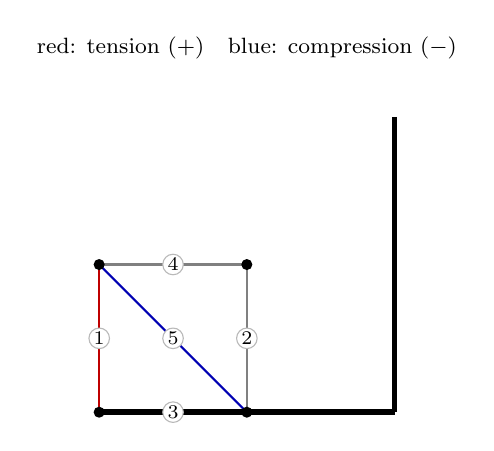
\begin{tikzpicture}[scale=1.250,>=Stealth,line join=round]
  \coordinate (P0) at (0.000,0.000);
  \coordinate (K) at (0.000,-3.000);
  \coordinate (C) at (-3.000,-3.000);
  \coordinate (TO1) at (-3.000,-1.500);
  \coordinate (TU0) at (-1.500,-3.000);
  \coordinate (TU1) at (-1.500,-1.500);
  \draw[thick,red!75!black] (C) -- (TO1);
  \draw[thick,gray] (TU0) -- (TU1);
  \draw[thick,red!75!black] (C) -- (TU0);
  \draw[thick,gray] (TO1) -- (TU1);
  \draw[thick,blue!70!black] (TU0) -- (TO1);
  \draw[line width=2pt] (P0) -- (K);
  \draw[line width=2pt] (K) -- (C);
  \fill (C) circle (1.6pt);
  \fill (TO1) circle (1.6pt);
  \fill (TU0) circle (1.6pt);
  \fill (TU1) circle (1.6pt);
  \node[circle,fill=white,draw=gray!55,inner sep=0.5pt,font=\scriptsize] at (-3.000,-2.250) {1};
  \node[circle,fill=white,draw=gray!55,inner sep=0.5pt,font=\scriptsize] at (-1.500,-2.250) {2};
  \node[circle,fill=white,draw=gray!55,inner sep=0.5pt,font=\scriptsize] at (-2.250,-3.000) {3};
  \node[circle,fill=white,draw=gray!55,inner sep=0.5pt,font=\scriptsize] at (-2.250,-1.500) {4};
  \node[circle,fill=white,draw=gray!55,inner sep=0.5pt,font=\scriptsize] at (-2.250,-2.250) {5};
  \node[font=\footnotesize] at (-1.50,0.70) {red: tension $(+)$\quad blue: compression $(-)$};
\end{tikzpicture}
\end{center}
\par\medskip\textbf{4.\ Section-force diagrams of the beams}\par
\begin{center}
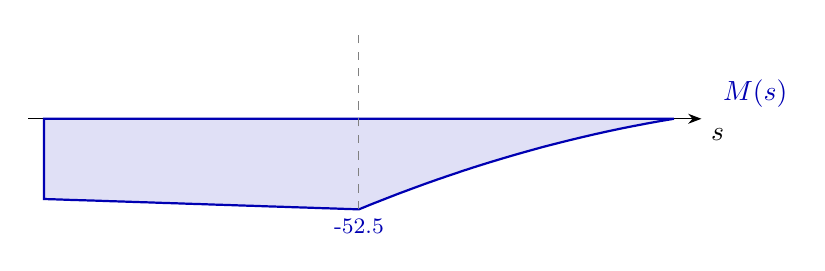
\begin{tikzpicture}[>=Stealth]
  \draw[->] (-0.2,0) -- (8.35,0) node[below right]{$s$};
  \filldraw[fill=blue!70!black!12,draw=blue!70!black,thick] (0,0) -- plot coordinates {(0.000,-1.019) (0.167,-1.024) (0.333,-1.030) (0.500,-1.035) (0.667,-1.040) (0.833,-1.046) (1.000,-1.051) (1.167,-1.057) (1.333,-1.062) (1.500,-1.068) (1.667,-1.073) (1.833,-1.079) (2.000,-1.084) (2.167,-1.090) (2.333,-1.095) (2.500,-1.101) (2.667,-1.106) (2.833,-1.112) (3.000,-1.117) (3.167,-1.123) (3.333,-1.128) (3.500,-1.134) (3.667,-1.139) (3.833,-1.145) (4.000,-1.150) (4.000,-1.150) (4.167,-1.082) (4.333,-1.017) (4.500,-0.952) (4.667,-0.890) (4.833,-0.829) (5.000,-0.770) (5.167,-0.713) (5.333,-0.657) (5.500,-0.603) (5.667,-0.551) (5.833,-0.501) (6.000,-0.452) (6.167,-0.405) (6.333,-0.359) (6.500,-0.316) (6.667,-0.274) (6.833,-0.234) (7.000,-0.195) (7.167,-0.158) (7.333,-0.123) (7.500,-0.090) (7.667,-0.058) (7.833,-0.028) (8.000,0.000)} -- (8.000,0) -- cycle;
  \draw[gray,dashed,thin] (4.000,-1.15) -- (4.000,1.15);
  \node[below,blue!70!black,font=\footnotesize] at (4.000,-1.150) {-52.5};
  \node[blue!70!black,right] at (8.50,0.32) {$M(s)$};
\end{tikzpicture}\\[5pt]
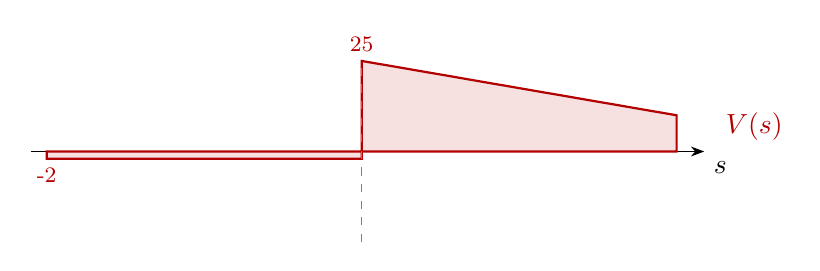
\begin{tikzpicture}[>=Stealth]
  \draw[->] (-0.2,0) -- (8.35,0) node[below right]{$s$};
  \filldraw[fill=red!70!black!12,draw=red!70!black,thick] (0,0) -- plot coordinates {(0.000,-0.092) (0.167,-0.092) (0.333,-0.092) (0.500,-0.092) (0.667,-0.092) (0.833,-0.092) (1.000,-0.092) (1.167,-0.092) (1.333,-0.092) (1.500,-0.092) (1.667,-0.092) (1.833,-0.092) (2.000,-0.092) (2.167,-0.092) (2.333,-0.092) (2.500,-0.092) (2.667,-0.092) (2.833,-0.092) (3.000,-0.092) (3.167,-0.092) (3.333,-0.092) (3.500,-0.092) (3.667,-0.092) (3.833,-0.092) (4.000,-0.092) (4.000,1.150) (4.167,1.121) (4.333,1.093) (4.500,1.064) (4.667,1.035) (4.833,1.006) (5.000,0.978) (5.167,0.949) (5.333,0.920) (5.500,0.891) (5.667,0.862) (5.833,0.834) (6.000,0.805) (6.167,0.776) (6.333,0.747) (6.500,0.719) (6.667,0.690) (6.833,0.661) (7.000,0.632) (7.167,0.604) (7.333,0.575) (7.500,0.546) (7.667,0.517) (7.833,0.489) (8.000,0.460)} -- (8.000,0) -- cycle;
  \draw[gray,dashed,thin] (4.000,-1.15) -- (4.000,1.15);
  \node[above,red!70!black,font=\footnotesize] at (4.000,1.150) {25};
  \node[below,red!70!black,font=\footnotesize] at (0.000,-0.092) {-2};
  \node[red!70!black,right] at (8.50,0.32) {$V(s)$};
\end{tikzpicture}\\[5pt]
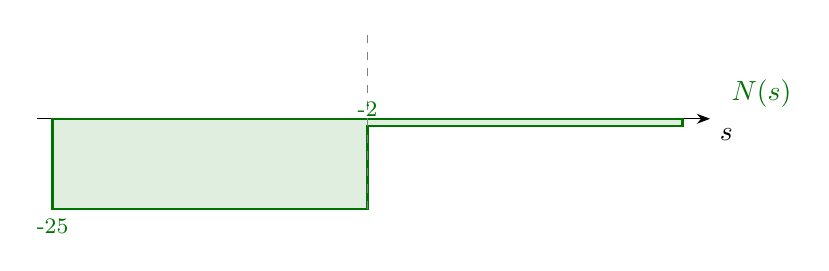
\begin{tikzpicture}[>=Stealth]
  \draw[->] (-0.2,0) -- (8.35,0) node[below right]{$s$};
  \filldraw[fill=green!45!black!12,draw=green!45!black,thick] (0,0) -- plot coordinates {(0.000,-1.150) (0.167,-1.150) (0.333,-1.150) (0.500,-1.150) (0.667,-1.150) (0.833,-1.150) (1.000,-1.150) (1.167,-1.150) (1.333,-1.150) (1.500,-1.150) (1.667,-1.150) (1.833,-1.150) (2.000,-1.150) (2.167,-1.150) (2.333,-1.150) (2.500,-1.150) (2.667,-1.150) (2.833,-1.150) (3.000,-1.150) (3.167,-1.150) (3.333,-1.150) (3.500,-1.150) (3.667,-1.150) (3.833,-1.150) (4.000,-1.150) (4.000,-0.092) (4.167,-0.092) (4.333,-0.092) (4.500,-0.092) (4.667,-0.092) (4.833,-0.092) (5.000,-0.092) (5.167,-0.092) (5.333,-0.092) (5.500,-0.092) (5.667,-0.092) (5.833,-0.092) (6.000,-0.092) (6.167,-0.092) (6.333,-0.092) (6.500,-0.092) (6.667,-0.092) (6.833,-0.092) (7.000,-0.092) (7.167,-0.092) (7.333,-0.092) (7.500,-0.092) (7.667,-0.092) (7.833,-0.092) (8.000,-0.092)} -- (8.000,0) -- cycle;
  \draw[gray,dashed,thin] (4.000,-1.15) -- (4.000,1.15);
  \node[above,green!45!black,font=\footnotesize] at (4.000,-0.092) {-2};
  \node[below,green!45!black,font=\footnotesize] at (0.000,-1.150) {-25};
  \node[green!45!black,right] at (8.50,0.32) {$N(s)$};
\end{tikzpicture}\\[10pt]
\end{center}
\end{document}